\documentclass[a4paper,twoside]{article}
\usepackage{blindtext}  
\usepackage{geometry}

% Chinese support
\usepackage[UTF8, scheme = plain]{ctex}

% Page margin layout
\geometry{left=2.3cm,right=2cm,top=2.5cm,bottom=2.0cm}


\usepackage{listings}
\usepackage{xcolor}
\usepackage{geometry}
\usepackage{amsmath}
\usepackage{float}
\usepackage{hyperref}

\usepackage{graphics}
\usepackage{graphicx}
\usepackage{subcaption}
\usepackage{epsfig}
\usepackage{float}

\usepackage{algorithm}
\usepackage[noend]{algpseudocode}

\usepackage{booktabs}
\usepackage{threeparttable}
\usepackage{longtable}
\usepackage{tikz}
\usepackage{multicol}

% cite package, to clean up citations in the main text. Do not remove.
\usepackage{cite}

\usepackage{color,xcolor}

%% The amssymb package provides various useful mathematical symbols
\usepackage{amssymb}
%% The amsthm package provides extended theorem environments
\usepackage{amsthm}
\usepackage{amsfonts}
\usepackage{enumerate}
\usepackage{enumitem}
\usepackage{listings}
\usepackage{minted}


\usepackage{indentfirst}
\setlength{\parindent}{2em} % Make two letter space in the first paragraph
\usepackage{setspace}
\linespread{1.5} % Line spacing setting
\usepackage{siunitx}
\setlength{\parskip}{0.5em} % Paragraph spacing setting

% \usepackage[contents =22920202204622, scale = 10, color = black, angle = 50, opacity = .10]{background}

\renewcommand{\figurename}{图}
\renewcommand{\listingscaption}{代码}
\renewcommand{\tablename}{表格}
\renewcommand{\contentsname}{目录}
\floatname{algorithm}{算法}

\graphicspath{ {images/} }

%%%%%%%%%%%%%
\newcommand{\StudentNumber}{22920202204622}  % Fill your student number here
\newcommand{\StudentName}{熊恪峥}  % Replace your name here
\newcommand{\PaperTitle}{实验(二)词法分析器}  % Change your paper title here
\newcommand{\PaperType}{编译原理} % Replace the type of your report here
\newcommand{\Date}{2023年3月26日}
\newcommand{\College}{信息学院}
\newcommand{\CourseName}{编译原理}
%%%%%%%%%%%%%

%% Page header and footer setting
\usepackage{fancyhdr}
\usepackage{lastpage}
\pagestyle{fancy}
\fancyhf{}
% This requires the document to be twoside
\fancyhead[LO]{\texttt{\StudentName }}
\fancyhead[LE]{\texttt{\StudentNumber}}
\fancyhead[C]{\texttt{\PaperTitle }}
\fancyhead[R]{\texttt{第{\thepage}页,共\pageref*{LastPage}页}}


\title{\PaperTitle}
\author{\StudentName}
\date{\Date}

\algnewcommand\algorithmicinput{\textbf{Input:}}
\algnewcommand\algorithmicoutput{\textbf{Output:}}
\algnewcommand\Input{\item[\algorithmicinput]}%
\algnewcommand\Output{\item[\algorithmicoutput]}%

\newenvironment{longlisting}{\captionsetup{type=figure}}{}

\usetikzlibrary{positioning, shapes.geometric}

\begin{document}
	
%%%%%%%%%%%%%%%%%%%%%%%%%%%%%%%%%%%%%%%%%%%%
\makeatletter % change default title style
\renewcommand*\maketitle{%
	\begin{center} 
		\bfseries  % title 
		{\LARGE \@title \par}  % LARGE typesetting
		\vskip 1em  %  margin 1em
		{\global\let\author\@empty}  % no author information
		{\global\let\date\@empty}  % no date
		\thispagestyle{empty}   %  empty page style
	\end{center}%
	\setcounter{footnote}{0}%
}
\makeatother
%%%%%%%%%%%%%%%%%%%%%%%%%%%%%%%%%%%%%%%%%%%%
	
	
\thispagestyle{empty}

\vspace*{1cm}

\begin{figure}[htb]
	\centering
	
\includegraphics[width=4.0cm]{logo.png}
\end{figure}

\vspace*{1cm}

\begin{center}
	\Huge{\textbf{\PaperType}}
	
	\Large{\PaperTitle}
\end{center}

\vspace*{1cm}

\begin{table}[H]
	\centering	
	\begin{Large}
		\renewcommand{\arraystretch}{1.5}
		\begin{tabular}{p{3cm} p{5cm}<{\centering}}
			姓\qquad 名 & \StudentName  \\
			\hline
			学\qquad号 & \StudentNumber \\
			\hline
			日\qquad期 & \Date  \\
			\hline
			学\qquad院 & \College  \\
			\hline
			课程名称 & \CourseName  \\
			\hline
		\end{tabular}
	\end{Large}
\end{table}

\newpage

\title{
	\Large{\textcolor{black}{\PaperTitle}}
}
	
	
\maketitle
	
\tableofcontents
 
\newpage
\setcounter{page}{1}

\begin{spacing}{1.2}

\section{实验目的}

掌握词法分析器的构造原理,掌握手工编程或LEX编程方法之一。

\section{实验内容}

编写一个LEX源程序,使之生成一个词法分析器,能够把输入的源程序转换为词法单元序列输出。

\section{实现思路}

我既完成了手工编程,也完成了使用LEX编程实现。

使用手工编程,可以参考关键字、表达式等词法单元的定义,手工处理歧义等问题,对源代码识别。

使用LEX编程,需要写出准确的正则表达式,对源代码识别。在识别的过程中,可以执行指定的动作,在执行动作
时可以将识别的词法单元及其附加信息保存在结构体中构成一列表。再进行输出。
定义的词法单元正则表达式如代码~\ref{code:reg}。

\begin{listing}[htb]
	\caption{词法单元正则表达式}
	\label{code:reg}
	\begin{minted}{c}
delim    [ \t\r\n]
ws       {delim}+
letter   [A-Za-z]
digit    [0-9]
id       {letter}({letter}|{digit})*
number   {digit}+(\.{digit}+)?(E[+-]?{digit}+)?(f|lf|sz)?
eoc      \*\/
	\end{minted}
\end{listing}

运行效果如图~\ref{fig:run}。
\begin{figure}[htb]
	\centering
	\caption{运行结果}
	\label{fig:run}
	\begin{subfigure}[b]{0.4\textwidth}
		\centering
		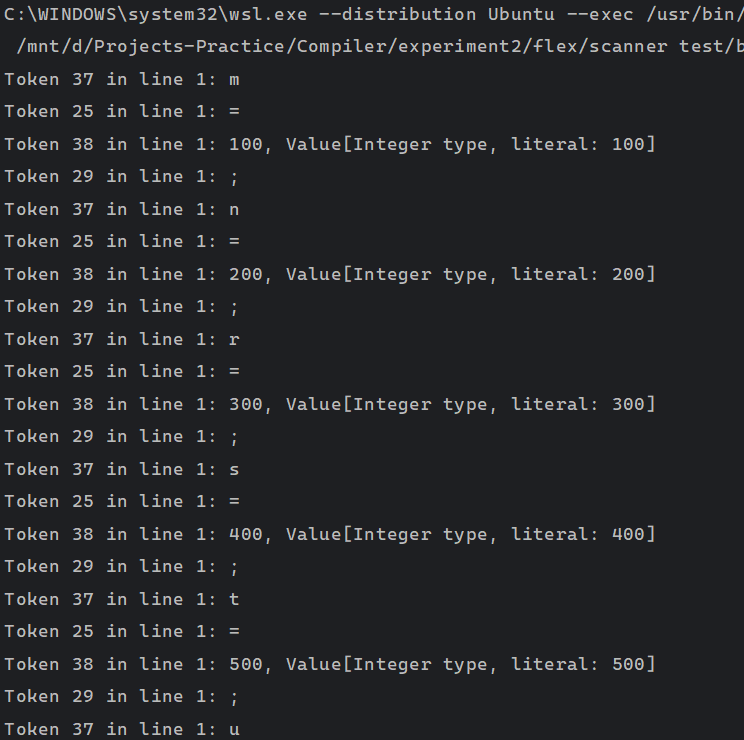
\includegraphics[width=0.9\textwidth]{images/lex.png}
		\caption{使用lex}
	\end{subfigure}
	\begin{subfigure}[b]{0.4\textwidth}
		\centering
		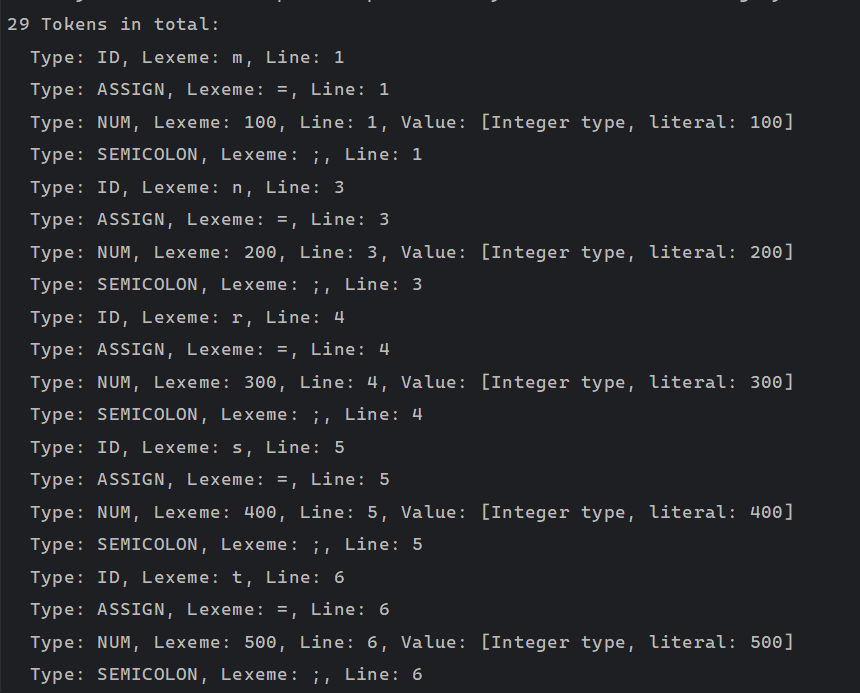
\includegraphics[width=0.9\textwidth]{images/byhand.png}
		\caption{手工编写}
	\end{subfigure}
\end{figure}

\section{问题一、如何良好地处理嵌套块注释?}

良好地处理嵌套注释不仅能正确地忽略注释内容,还能对不匹配的错误代码正常地报错。

嵌套块注释是一种常见的现象。在C语言中/* */是块注释,这一对符号
可以嵌套使用,处理时应当以最外层的块注释为准。

在识别块注释时,我们不但应当正确识别正确的块注释,还应当正确地识别错误的块注释,并且进行报错,
例如块注释开始符号少于结束符号、多于结束符号等状况。例如图~\ref{fig:ecom}展示了本次LEX实现中
对不匹配块注释的两种报错。
\begin{figure}[htb]
	\centering
	\caption{错误注释的情况}
	\label{fig:ecom}
	\begin{subfigure}[b]{0.4\textwidth}
		\centering
		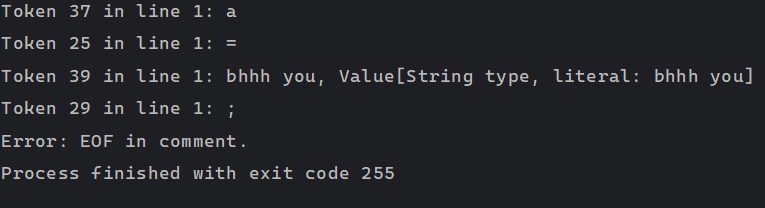
\includegraphics[width=0.9\textwidth]{images/morestart.png}
		\caption{缺少注释终止符(块注释开始符号多于结束符号)}
	\end{subfigure}
	\begin{subfigure}[b]{0.4\textwidth}
		\centering
		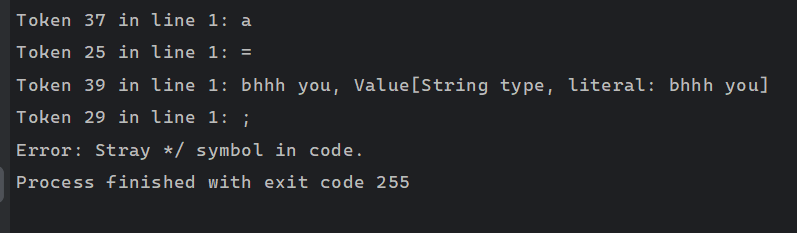
\includegraphics[width=0.9\textwidth]{images/moreend.png}
		\caption{缺少注释开始符号(块注释开始符号少于结束符号)}
	\end{subfigure}
\end{figure}
可见该分析器能正确识别错误并给出报错。

\subsection{正则表达式\textbf{不可能}良好地处理嵌套注释}

良好地处理嵌套注释不仅能正确地忽略注释内容,还能对不匹配的错误代码正常地报错。

最简单的处理嵌套注释的方式是使用正则表达式,如代码~\ref{eq:blockcommentreg}所示。
\begin{listing}[htb]
	\caption{处理嵌套注释正则表达式}
	\label{code:blockcommentreg}
	\begin{minted}{c}
		[\/][\*]([^\*])*[\*]([\*]|[^\*\/](([^\*])*)[\*])*(\/)
	\end{minted}
\end{listing}
然而,这种方式对错误的注释处理不够完善,例如处理串\texttt{/*aa/*bb*/*/*/}时会有多余
输出,如图~\ref{fig:errreg}。
\begin{figure}[htb]
	\centering
	\caption{错误注释的情况}
	\label{fig:errreg}
	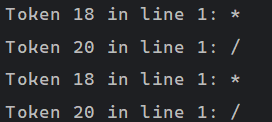
\includegraphics[width=0.4\textwidth]{images/errreg.png}
\end{figure}

这种现象产生的原因是源串中只有被/**/匹配对正确包含的bb会被作为注释匹配到,然后其它的元素则会被
其他规则匹配到,因而不能够正确识别这是一种错误,然后输出相应的、类似我的实现的、如图~\ref{fig:ecom}中的
错误消息。而在真实世界的编译器中,这一错误的Token序列会进入到后续的工作中,
最终因为不符合语法或者语义规则而报错。然而一旦将报错推迟到后续阶段,由于被部分删除的注释
和不完整的Token序列已经没有办法提供充足的信息来生成合理的、易读的、用户友好的错误报告,
因此这种方式有致命的缺陷。

在手工编写的Lexer中,可以使用了一个栈来处理注释开始符号的嵌套,当遇到注释开始符号时,将其入栈,遇到注释结束符号时,将其出栈,
当栈为空时,说明注释结束,否则说明注释未结束。
如果缺少注释终结符号,当文件到达EOF时,栈仍不为空,则可以针对性报错,如果缺少注释开始符号,当遇到注释结束符号时,栈为空,
则也可以针对性报错。仅仅使用正则表达式在这种情况下是无法处理的。那么使用flex如何生成一个能够良好处理嵌套注释的词法分析器呢?

\subsection{使用Start Condition良好地处理嵌套块注释}

Start condition是LEX提供的一种功能。它允许用户在词法分析器中定义多个状态,每个状态都有一个名字,当使用\texttt{BEGIN}
动作时可以激活一个start condition。此时,只有针对这一start condition的规则是有效的。为了给规则限定start condition,
可以在规则的前方进行声明。默认的、一进入LEX中的start condition是\texttt{INITIAL}。

为了处理嵌套注释,可以使用一个start condition,再定义特殊的规则,在这些规则的动作中维护栈的状态。这样就可以使用上述栈的方法
处理注释的嵌套。当嵌套注释处理完毕时,回到\texttt{INITIAL}环境,这样就能处理正确的嵌套注释。

而对于错误的嵌套注释,上述切换的过程给予我们足够的信息进行具有针对性的报错:
\begin{enumerate}
	\item 如果处在注释的start condition中,而且读到了\texttt{EOF},则说明缺少注释终止符号。
	\item 如果不在注释的start condition中,而且读到了\texttt{*/},则说明缺少注释开始符号。
\end{enumerate}
因此,借助start condition,我们可以很容易地实现良好地处理嵌套注释及其错误情况的报错。

此外,由于我们只需要判断是否栈空,因此进出栈的操作可以简化为变量的加减操作,这样可以减少内存访问的开销。

使用这一思路处理嵌套注释的LEX定义如代码~\ref{code:blockcomment}所示。
\begin{listing}[htb]
	\caption{处理嵌套注释正则表达式}
	\label{code:blockcomment}
	\begin{minted}{c}
%x COMMENT
%%
%{
   int _yycmtnest = 0;
%}
"/*"            { BEGIN(COMMENT); ++_yycmtnest;}
"//".*          /* // comments to end of line */
<COMMENT>[^*/]* /* Eat non-comment delimiters */
<COMMENT>"/*"   {++_yycmtnest;}
<COMMENT>"*/"   {if (--_yycmtnest == 0) BEGIN(INITIAL);}
<COMMENT>[*/]   /* Eat a / or * if it doesn't match comment sequence */
<COMMENT><<EOF>> { yyerror("EOF in comment."); }
{eoc}            { yyerror("Stray */ symbol in code."); }
%%
	\end{minted}
\end{listing}

以上代码实现了上述分析得出的所有必要的处理,能够实现如图~\ref{fig:ecom}中的错误报告。

注释这一在词法分析过程中
需要被移除的内容,可以在词法分析阶段完成所有的错误处理,并且有能力给出易读、准确的错误报告,这样对于嵌套注释
的处理才是正确、良好的。

\section{问题二、如何处理字符串常量}

处理字符串常量和处理注释类似,虽然不需要考虑嵌套的情况,但需要考虑当引号不匹配时如何正确地报告错误。

引号的错误也相对比较简单。由于使用相同的符号标记字符串的开始和结束,因此实质上的错误只有一种:
缺乏字符串的结束符。因为若多出一个引号,那么这个引号会被当作下一个字符串的开始,而不会被当作多出了字符串的结束符,
这样处理的合理性在于,在许多语言中两个相邻的字符串可以被合并为一个字符串,因此如此处理多出的引号更符合实践中的操作。

因此,仿照处理注释的方法,可以使用start condition来处理字符串常量。当遇到字符串常量的开始符号时,进入字符串常量的start condition,
如果在其中读到了EOF,则可以认为缺乏字符串的结束符。如代码~\ref{code:strlit}。
\begin{listing}[htb]
	\caption{问题二、如何处理字符串常量}
	\label{code:strlit}
	\begin{minted}{c}
%x STRING
%%
%{
   int _yycmtnest = 0;
%}
["]             { BEGIN(STRING);}
<STRING>[^"]*   { EMIT_TOKEN(TK_STRING); }
<STRING>["]     { BEGIN(INITIAL);}
<STRING><<EOF>> { yyerror("EOF in string."); }
%%
	\end{minted}
\end{listing}

\section{问题三、如何良好区分不同类型的字面量}

不同类别的字面量通常在语法分析阶段需要进行不同的处理,而在词法分析阶段有足够的信息可以对不同类型的字面量进行区分。

以上代码中出现了\texttt{EMIT\_TOKEN}宏,该宏定义进一步调用另外实现的
\texttt{create\_token}函数,对LEX处理出的词法单元文本进一步处理,
在这一过程中,可以对常量进行进一步的处理,以便于对不同类型的字面量进行不同的处理。

\begin{listing}[htb]
	\caption{区分不同类型的字面量}
	\label{code:token}
	\begin{minted}{c}
extern "C" void *create_token(token_type t, const char *s, int l)
{
	string lexeme{s};
	if (t != TK_NUM && t != TK_STRING){
		return new token{t, lexeme, l, {}};
	}else{
		if (t == TK_NUM){
			bool floating = false;
			for (char p: lexeme){
				if (p == '.'){
					floating = true;
					break;
				}
			}
			if (floating){
				return new token{t, lexeme, l, {stod(lexeme)}};
			}else{
				return new token{t, lexeme, l, {stoi(lexeme)}};
			}
		}else{
			return new token{t, lexeme, l, {lexeme}};
		}
	}
}
	\end{minted}
\end{listing}

对于TK\_STRING类型,可以不做特殊处理,也可以做特殊处理:将其中符合转义规则的部分进行替换。在这里不做处理。对于TK\_NUM类型的Token,它可能携带整数,也可能携带浮点数。因此,可以进一步扫描字面量的文本。例如科学计数法、
小数点、类型后缀的部分均可以提示其类型。然后,可以使用共用体在存储Token信息的结构体中,进一步保存经过正确转换
的数值。

这一部分的实现如代码~\ref{code:token}所示。这里使用了C++11引入的\texttt{std::variant}来代替传统C语言的共用体。
它可以记录类型信息,并根据其类型获取值,使得程序编写更为便利。


\section{对手工编写和LEX生成优劣的讨论}

在本次实验中,我分别使用手工编写与LEX生成的方式对一种语言的词法分析器进行编写。我认为,手工编写
和LEX生成分别有如下优点:

手工生成
\begin{itemize}
	\item 更灵活自由
	\item 能够更方便地实现复杂嵌套块的分析
	\item 更容易提供良好的错误信息
\end{itemize}

LEX生成
\begin{itemize}
	\item 简洁直观
	\item 更容易保证正确性
\end{itemize}

从实践的视角来看,在工业界得以广泛应用的编译器,通常具有手工编写的词法分析器和语法分析器,
因为真实世界的使用要求效率,就要求给出较好的错误信息,并且往往面临着复杂的语法结构,因此需要更大的
灵活性和自由度。而学术性更强的语言,例如Scala、OCaml等语言通常使用LEX生成的词法分析器,因为这样一来
可以忽略实现细节、直接使用规则生成对应的词法分析器。因而能够更方便地对各种特性进行研究和讨论,而不
受限于具体的实现细节。

从历史的视角来看,随着一门编程语言从实验室走到日常使用的环境中去,其词法分析器和语法分析器通常都会从
工具生成的方式走向手工编写。例如GCC,早期版本的GCC使用生成的词法分析和语法分析器。随着实际的使用中
暴露的问题,例如不够友好地错误信息,日渐复杂的语法定义和对性能的要求;以及竞争对手Clang使用手工编写
的词法分析和语法分析所带来的良好体验,从3.x版本开始\footnote[1]{\url{https://gcc.gnu.org/wiki/New_C_Parser}},GCC的词法分析
和语法分析被替换成了手工编写的版本。这一过程持续了十多年,直到GCC 4.0版本,这一过程才正式完成。

手工编写的优势不仅体现在错误处理和恢复上,更体现在对复杂语言特性的处理上,这是由于其灵活自由的特点决定的。
使用工具生成则缺乏这一特点,例如工具必须严格地使用正则描述词法规则,使用上下文无关文法描述语法规则。这一过程中,词法分析和语法分析
严格分开。但是,面对复杂的语言特性,比如C++中的模板特性,
当嵌套模板发生时,例如\texttt{std::vector<std::vector<int>>},这时候“如何判断\texttt{>>}是一个Token还是两个Token”就成了一个问题。
而解决这一问题,再复杂的正则、表达能力再强的语法都不如使语法分析和词法分析共同进行、互相使用对方的中间状态来的更为可行。
然而,一旦使用了工具生成,就很难做到这一点。

当然,在面对实际的问题时,常常比起“哪一种方案更有学术上的正确性”,更需要确定“哪一种方案的正外部性和负外部性综合而言更能令人接受”。
即使手工编写可能不如正则表达式直接定义来得正确、精准,从这一点出发,我认为手工编写和LEX生成的优劣并不是一个绝对的问题,而应当
具有同等重要的地位、应当面向实际的需求做出正确的trade-off,选择最合适的方案。



\clearpage
\appendix
\section{附录A、完整的LEX定义}
\begin{longlisting}
	\caption{完整的LEX定义}
	\label{code:fullcode}
	\begin{minted}{c}
%{
#include <stdio.h>
#include <stdlib.h>

#include "lexer.h"

#define EMIT_TOKEN(type) yylval=create_token(type,yytext,yylineno); return (type);

struct token* yylval;
int yylines=0;

static void yyerror(char *msg)
{
    fprintf(stderr, "Error: %s", msg);
    exit(-1);
}

%}

delim    [ \t\r\n]
ws       {delim}+
letter   [A-Za-z]
digit    [0-9]
id       {letter}({letter}|{digit})*
number   {digit}+(\.{digit}+)?(E[+-]?{digit}+)?(f|lf|sz)?
eoc      \*\/

%x COMMENT
%x STRING

%%
%{
   int _yycmtnest = 0;
%}
"/*"            { BEGIN(COMMENT); ++_yycmtnest;}
"//".*          /* // comments to end of line */
<COMMENT>[^*/]* /* Eat non-comment delimiters */
<COMMENT>"/*"   {++_yycmtnest;}
<COMMENT>"*/"   {if (--_yycmtnest == 0) BEGIN(INITIAL);}
<COMMENT>[*/]   /* Eat a / or * if it doesn't match comment sequence */
<COMMENT><<EOF>> { yyerror("EOF in comment."); }
{eoc}            { yyerror("Stray */ symbol in code."); }

["]             { BEGIN(STRING);}
<STRING>[^"]*   { EMIT_TOKEN(TK_STRING); }
<STRING>["]     { BEGIN(INITIAL);}
<STRING><<EOF>> { yyerror("EOF in string."); }

{ws}       { /*no action and no return */ }
if         { EMIT_TOKEN(TK_IF); }
while      { EMIT_TOKEN(TK_WHILE);}
do         { EMIT_TOKEN(TK_DO);}
break      { EMIT_TOKEN(TK_BREAK);}
true       { EMIT_TOKEN(TK_TRUE); }
false      { EMIT_TOKEN(TK_FALSE);}
int        { EMIT_TOKEN(TK_INT);  }
char       { EMIT_TOKEN(TK_CHAR);  }
bool       { EMIT_TOKEN(TK_BOOL); }
float      { EMIT_TOKEN(TK_FLOAT); }

{id}       { EMIT_TOKEN(TK_ID); }
{number}   { EMIT_TOKEN(TK_NUM); }

\(         { EMIT_TOKEN(TK_LPAREN);}
\)         { EMIT_TOKEN(TK_RPAREN);}
\]         { EMIT_TOKEN(TK_LBRACKET); }
\[         { EMIT_TOKEN(TK_RBRACKET); }
\{         { EMIT_TOKEN(TK_LBRACE); }
\}         { EMIT_TOKEN(TK_RBRACE); }


";"        { EMIT_TOKEN(TK_SEMICOLON); }
","        { EMIT_TOKEN(TK_COMMA); }
"+"        { EMIT_TOKEN(TK_PLUS); }
"-"        { EMIT_TOKEN(TK_MINUS); }
"*"        { EMIT_TOKEN(TK_MULTIPLY); }
"/"        { EMIT_TOKEN(TK_DIVIDE); }
"<"        { EMIT_TOKEN(TK_LT); }
"<="       { EMIT_TOKEN(TK_LTE); }
"=="       { EMIT_TOKEN(TK_ASSIGN); }
"="        { EMIT_TOKEN(TK_EQ); }
"!="       { EMIT_TOKEN(TK_NEQ); }
">"        { EMIT_TOKEN(TK_GT); }
">="       { EMIT_TOKEN(TK_GTE); }

.          { yyerror("Unexpected character.");}
%%

int yywrap()
{
    return 1;
}
	\end{minted}
\end{longlisting}

\clearpage

\section{附录B、完整的手工实现}

\begin{longlisting}
	\caption{完整的手工实现}
	\label{code:fullcode}
	\begin{minted}{c}
#include <format>
#include <iostream>

#include "lexer.h"

using namespace std;

std::vector<token> scanner::scan()
{
	while (!is_end())
	{
		start_ = current_;
		scan_next();
	}

	tokens_.emplace_back(token_type::EOF_TOKEN, "", line_);
	return tokens_;
}

void scanner::scan_next()
{
	char c = advance();
	switch (c)
	{
	case '(':
		add_token(token_type::LPAREN);
		break;
	case ')':
		add_token(token_type::RPAREN);
		break;
	case '[':
		add_token(token_type::LBRACKET);
		break;
	case ']':
		add_token(token_type::RBRACKET);
		break;
	case '{':
		add_token(token_type::LBRACE);
		break;
	case '}':
		add_token(token_type::RBRACE);
		break;
	case ',':
		add_token(token_type::COMMA);
		break;
	case '-':
		if (match('-'))
		{
			add_token(token_type::DMINUS);
		}
		else
		{
			add_token(token_type::MINUS);
		}
		break;
	case '+':
		if (match('+'))
		{
			add_token(token_type::DPLUS);
		}
		else
		{
			add_token(token_type::PLUS);
		}
		break;
	case ';':
		add_token(token_type::SEMICOLON);
		break;
	case '*':
		if (match('*'))
		{
			add_token(token_type::POWER);
		}
		else
		{
			add_token(token_type::MULTIPLY);
		}
		break;
	case '!':
		add_token(match('=') ? token_type::NEQ : token_type::NOT);
		break;
	case '=':
		add_token(match('=') ? token_type::EQ : token_type::ASSIGN);
		break;
	case '<':
		add_token(match('=') ? token_type::LTE : token_type::LT);
		break;
	case '>':
		add_token(match('=') ? token_type::GTE : token_type::GT);
		break;

	case '/':
		if (match('/')) // this is a line comment
		{
			consume_line_comment();
		}
		else if (match('*')) // this is a block comment
		{
			consume_block_comment();
		}
		else
		{
			add_token(token_type::DIVIDE);
		}
		break;

	case ' ':
	case '\r':
	case '\t':
		// Do nothing to ignore whitespaces.
		break;

	case '\n':
		line_++;
		break;

	case '"':
		scan_string();
		break;

	default:
		if (is_number_literal_component(c))
		{
			scan_number_literal();
		}
		else if (is_identifier_component(c))
		{
			scan_identifier();
		}
		else
		{
			cerr << format("Unexpected character {}.", c) << endl;
		}

		break;
	}
}

void scanner::scan_string()
{
	while (peek() != '"' && !is_end())
	{
		if (peek() == '\n')
		{
			line_++;
		}
		advance();
	}

	if (is_end())
	{
		cerr << "Unterminated string." << endl;
		return;
	}

	advance(); // eat the closing "

	auto lexeme = whole_lexeme();
	add_token(token_type::STRING, lexeme.substr(1, lexeme.size() - 2));
}

void scanner::scan_number_literal()
{
	while (is_number_literal_component(peek()))
		advance();

	bool floating{false};
	if (peek() == '.' && is_number_literal_component(peek(1)))
	{
		floating = true;
		advance();
		while (is_number_literal_component(peek()))
			advance();
	}

	if (floating)
	{
		add_token(token_type::NUM, stod(whole_lexeme()));
	}
	else
	{
		add_token(token_type::NUM, stoi(whole_lexeme()));
	}
}

void scanner::scan_identifier()
{
	while (is_identifier_component(peek()))
		advance();

	auto text = whole_lexeme();
	auto keyword = keywords_to_type_.find(text);

	if (keyword != keywords_to_type_.end())
	{
		add_token(keywords_to_type_[text]);
	}
	else
	{
		add_token(token_type::ID);
	}
}

void scanner::consume_block_comment()
{
	while (!is_end())
	{
		auto c = advance();
		if (c == '\n')
		{
			line_++;
		}
		else if (c == '*' && peek() == '/')
		{
			[[maybe_unused]]auto _ = advance(); // eat "/"
			return;
		}
		else if (c == '/' && peek() == '*') // nested block comment
		{
			[[maybe_unused]]auto _ = advance(); // eat "*"
			consume_block_comment();
		}
	}

	// not enough code to find next close sign */, so it's an error
	if (is_end())
	{
		cerr << "Unterminated block comment." << endl;
	}
}

void scanner::consume_line_comment()
{
	while (peek() != '\n' && !is_end())
		advance();
}

void scanner::add_token(token_type t)
{
	tokens_.emplace_back(t, whole_lexeme(), line_);
}

void scanner::add_token(token_type t, const literal_type &lit)
{
	tokens_.emplace_back(t, whole_lexeme(), line_, lit);
}
	\end{minted}
\end{longlisting}

\end{spacing}

\end{document}